\label{sec:experiments}


\begin{figure}[t]
  \centering
%   \vspace{-0.1cm} 
  % \setlength{\abovecaptionskip}{0cm} 
%   \setlength{\belowcaptionskip}{-0.05cm} 
  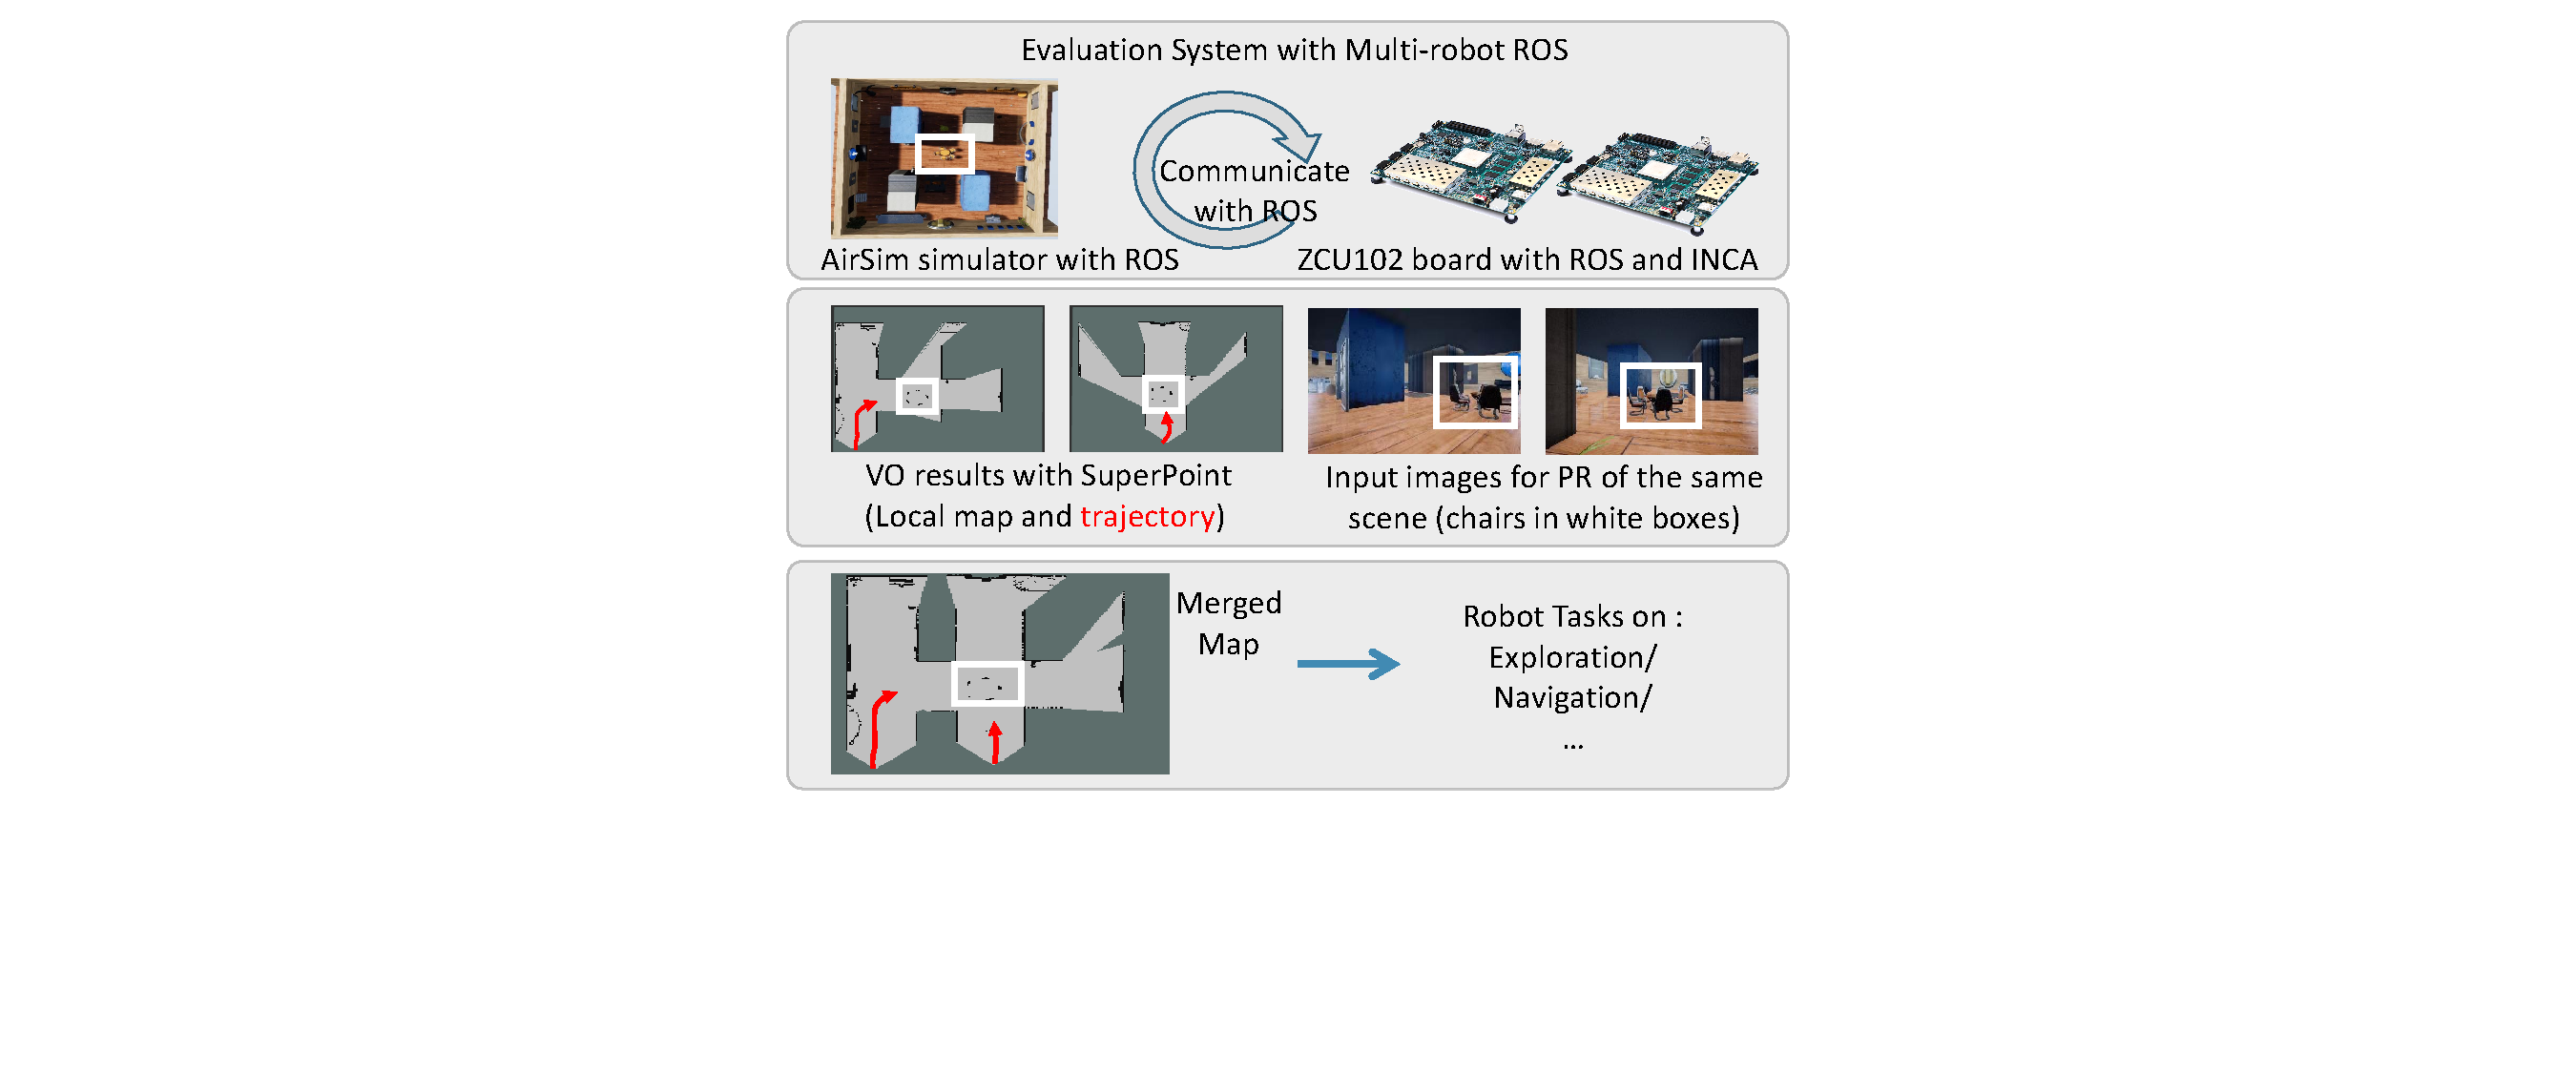
\includegraphics[width=0.8\linewidth]{fig/env.pdf}
  \caption{Multi-robot exploration: environment and results. }
  \label{fig:env}
\end{figure}


% In this section, the evaluation of the instruction-based-interruption, hardware modules for FE post-processing, and the overall MR-Exploration system are presented and analyzed.



\subsection{ Experiment Setup }

The hardware-in-loop evaluate environment is illustrated in \Cref{fig:env}(a). There is a simulation server providing the simulation environment based on AirSim  ~\cite{shah2018airsim}, which is a high-fidelity visual and physical simulation for autonomous vehicles. The AirSim simulation server provides the camera data for each agent. Two Xilinx ZCU102 boards  ~\cite{zcu102}, with ZU9 MPSoC  ~\cite{MPSoC}, are responsible for the calculation of each agent. 
The components in \Cref{fig:maexp} for each agent are implemented in the ZCU102 board. The implementation of the FE (\textcircled{1} in \Cref{fig:maexp}), SuperPoint ~\cite{detone2018superpoint}), are introduced in former sections. GeM  ~\cite{radenovic2018fine} is used to implement the PR module (\textcircled{2}). GeM is a CNN-based method with ResNet101 \cite{he2016deep} as the backbone, and the post-processing of GeM calculates the 3-norm of the output featuremaps.
The VO module (\textcircled{3}) in the experiment is the PnP  ~\cite{LepetitMoreno-Noguer-EPnP} method, which is widely used in the feature-point based VO. 
% including the open source the ORB-SLAM  ~\cite{Mur-Artal:2017281}. 
The DOpt module (\textcircled{4}) is proposed in  ~\cite{Choudhary:2017e66} and also used in former distributed SLAM system ~\cite{cieslewski2018data}. 
The Map Merging  ~\cite{Andre2014} (\textcircled{5}), Exploration  ~\cite{8202319} (\textcircled{6}), and Navigation  ~\cite{tbd} (\textcircled{7}) in this work are provided by the ROS framework. 

The hardware resources are listed in \Cref{tab:hardware}. The hardware resources are provided by Vivado after hardware implementation. Vivado\cite{Vivado} is the development toolchain for MPSoC provided by Xilinx. The CNN backbone is calculated by the Angel-Eye CNN accelerator ~\cite{guo2017angel} on the FPGA side of ZCU102 (Programmable logic, PL side). The FE post-processing steps run on our proposed accelerators, also on the PL side. The PL side has 2 clock frequencies. The CNN accelerator and the IAU are running at 300MHz. The accelerator for FE post-processing is running at 200MHz. Compared with the CNN accelerator, IAU and FE post-processing use very little hardware resources.

% % Table generated by Excel2LaTeX from sheet 'Sheet1'
% \begin{table}[t]
%   \centering
%   % \setlength{\abovecaptionskip}{2pt}
%   \caption{Hardware consumption of the proposed hardware}
% % Table generated by Excel2LaTeX from sheet 'Sheet1'
% \begin{tabular}{|c|c|c|c|c|}
%   \hline
%         & $\# DSP$ & $\# LUT$ & $\# FF$ & $\# BRAM$ \\
%   \hline
%   On-Board resource &   2520   &  274080      &  548160     & 912 \\
%   \hline
%   CNN accelerator &   1282   &  74569      &   171416    & 499 \\
%   \hline
%   IAU &   0   &  2268      &   4633    & 4 \\
%   \hline
%   FE post-processing & 25      &  17573     &   29115    & 10 \\
%   \hline
%   \end{tabular}%
  
%   \label{tab:hardware}%
% \end{table}%

\begin{figure}[t]
  \centering
%   \vspace{-0.1cm} 
  % \setlength{\abovecaptionskip}{0cm} 
%   \setlength{\belowcaptionskip}{-0.05cm} 
  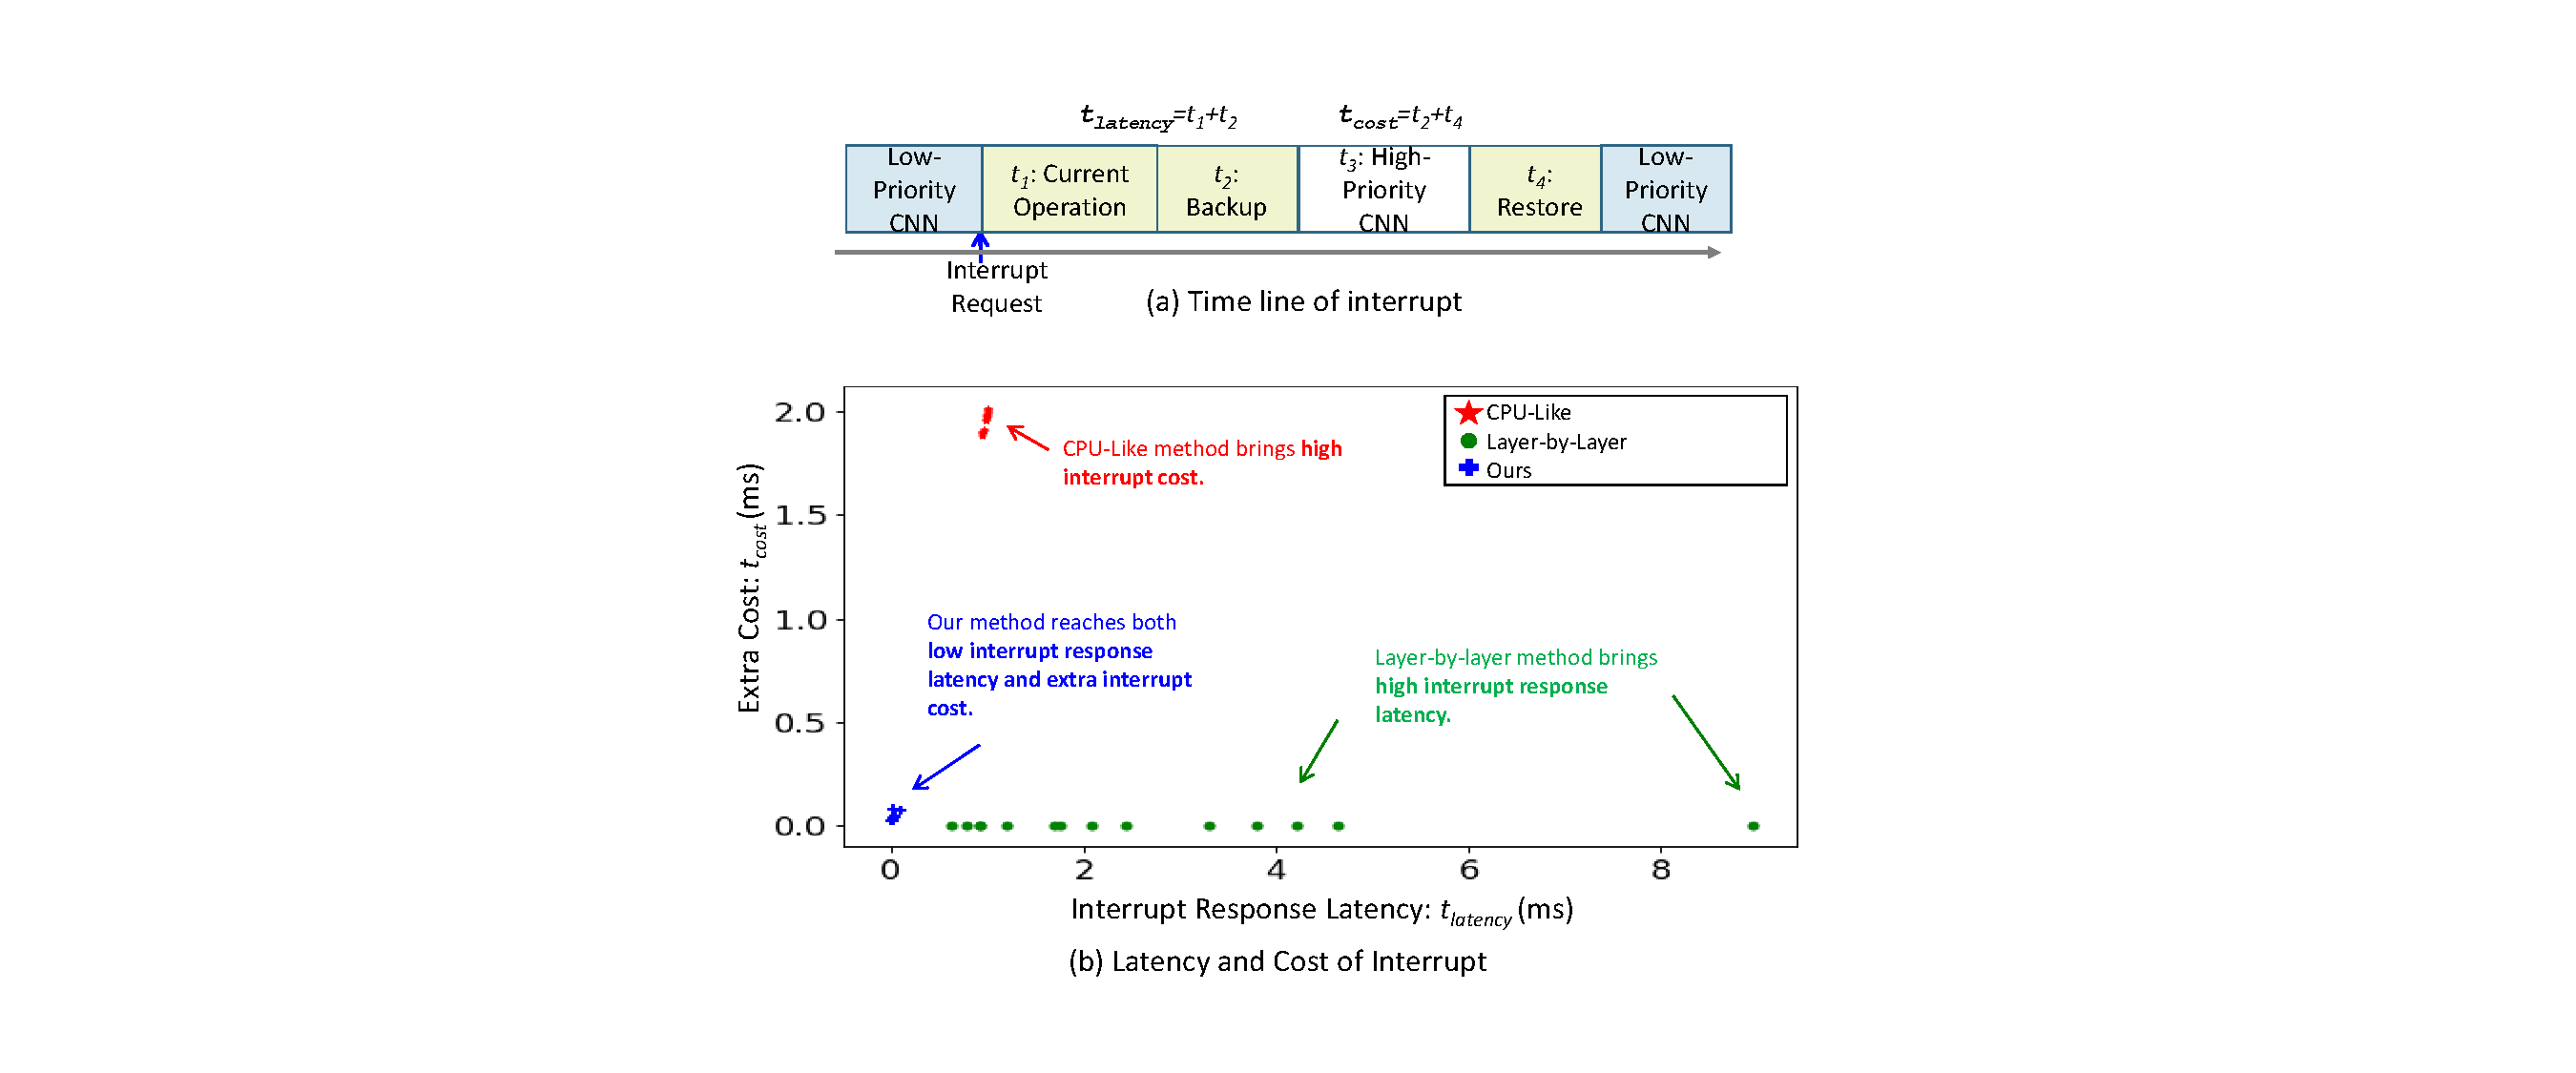
\includegraphics[width=0.99\linewidth]{fig/PRresult.pdf}
  \caption{The interrupt response latency \& extra time cost.}
  \label{fig:scatter1024}
\end{figure}


\subsection{Virtual Instruction-based interrupt }

\subsubsection{ Interrupt response latency and extra cost}


We evaluate the latency to respond the interrupt and the performance degradation of different interrupt method. In MR-Exploration, only the low-priority PR task is interruptible, and the interrupt position is unpredictable. GeM  ~\cite{radenovic2018fine} is used to implement the PR module in the experiment.
The CNN backbone of the GeM is ResNet101  ~\cite{he2016deep}, which contains 101 convolution layers. The input shape of the CNN is $480 \times 640 \times 3$. The parallelism of the Angel-Eye is $Para_{height}=8$, $Para_{in}=16$, $Para_{out}=16$, i.e. each CALC instruction processes 8 lines from 16 input channels to 16 output channels. 
% Thus, we randomly selected some interrupt locations inside the PR network.

As shown in \Cref{fig:scatter1024}(a), the latency to respond the interrupt in CPU-like method consists of the time to finish current executing instruction and the data backup time ($t_{latency} = t_1+t_2$) for the on-chip data/weights caches (totally 2.2MB). The latency in layer-by-layer interrupt is the time to finish current layer. The latency of our virtual-instruction-based method is the time to finish current executing instruction and the backup time for the calculated output results. 

The cost of CPU-like interrupt is the data transfer time of all the on-chip caches (totally 2.2MB) to/from DDR ($t_{cost} = t_2+t_4$). The cost of virtual-instruction-based method is only the recovery of the input/weights from DDR to on-chip caches ($t_{cost} = t_4$). There is no extra cost for the layer-by-layer interrupt.

% For a precise evaluation the CNN run time, we record the clock cycles of the beginning and end of each instruction. The time of the interrupt response latency and the total cost in the following evaluation is calculated from the clock cycles and the clock frequence.


We randomly sample 12 positions of the ResNet101 CNN backbone. The interrupt response latency and the extra time cost for different implementation of interrupt at the positions are listed in \Cref{fig:scatter1024}(b).
The CPU-like interrupt consumes the most extra cost ($t_{cost}$). Though the layer-by-layer interrupt consumes no extra time, the latency is much higher than our virtual-instruction-based interrupt. 
This is because the layer-by-layer interrupt need to wait for completion of a layer. The performance at same interrupt position in our proposed virtual interrupt can interrupt inside a layer, with lower latency.

Furthermore, though the network structures differ between different CNNs, the convolutional layers, which are the basic component in CNN, are similar between different CNNs. INCA monitors the running status inside each layer, and the interrupt respond latency and extra cost are only relevant to the currently operating layer. Thus, the latency and cost are also similar between different CNNs. In conclusion, the process for different CNN tasks are similar, and the cost of different tasks are similar.

% \subsubsection{ Time comparison between $t_1$ and $t_2$ }

% As described in \Cref{sec:virtualinstr}, the Layer-By-Layer interrupt method do not need to backup data before interruption ($t_2 = 0$). Though our Virtual-Instruction method (VI method) need to spend time to backup the final results, which are already generated yet not stored to DDR ($t_2$). However, compared with computation, the time of data backup ($t_2$) is short. We list the backup time and the convolution time ($t_1$) at some of the interrupt position in \Cref{fig:scatter1024}(b), with different featuremap shape, kernel size, and input/output channels. $H$, $W$ are the height, width of input featuremaps. $Ch_{in}$, $Ch_{out}$ are the number of input and output channels. The time of backup and calculation is listed in $Backup$ and $Conv$ columns. The ratio of backup and calculation are listed in the last column. The backup operation only consumes less than 20\% of the calculation time. For the first layer (first line of \Cref{tab:timecompare}). The input channels number is too small, so the calculation time is also short. Therefore, the backup time has reached half of the calculation time. 

% % Table generated by Excel2LaTeX from sheet 'Sheet4'
% \begin{table}[t]
%   \centering
%   % \footnotesize
%   \caption{Time comparison between data backup and calculation}
%     \begin{tabular}{|c|c|c|c|c|c|c|c|}
%     \hline
%     \multirow{2}[2]{*}{$H$} & \multirow{2}[2]{*}{$W$} & \multirow{2}[2]{*}{$Ch_{in}$} & \multirow{2}[2]{*}{$Ch_{out}$} & Kernel & Backup & Conv  & \multirow{2}[2]{*}{$\frac{Backup}{Conv}$} \bigstrut[t]\\
%           &       &       &       & Size  & ($t_2$,$us$)  & ($t1$,$us$)  &  \\
%     \hline
%     480   & 640   & 3     & 64    & $7 \times 7$ & 26.29  & 52.38  & 50.2\% \\
%     \hline
%     120   & 160   & 128   & 128   & $3 \times 3$ & 8.77  & 41.18  & 21.3\% \\
%     \hline
%     30    & 40    & 1024  & 2048  & $1 \times 1$ & 1.25  & 8.75  & 14.3\% \\
%     \hline
%     30    & 40    & 512   & 512   & $3 \times 3$ & 1.42  & 39.36  & 3.6\% \\
%     \hline
%     16    & 20    & 512   & 512   & $3 \times 3$ & 0.75  & 20.16  & 3.8\% \\
%     \hline
%     \end{tabular}%
%   \label{tab:timecompare}%
% \end{table}%


\subsection{ ROS based MR-Exploration }

The results of the Multi-Robot Exploration based on INCA is shown in \Cref{fig:env}. The space in the AirSim~\cite{shah2018airsim} for the robots to explore is shown in \Cref{fig:env}(a). It is a simple rectangle area with four different pillars, and some chairs at the center (in the white box).  \Cref{fig:env}(b) shows how PR works for map merging. The FE and VO of each agent produce the local map and trajectory on each ZCU102 board. When the PR threads on different agents find out a similar scene, the relative pose of the two agents at the similar scene is calculated. The map and the trajectory is merged with the calculated relative pose, as shown in \Cref{fig:env}(c).

In this example, the FE and PR are both executed on the same Angel-Eye accelerator. The frequency of the input camera is 20fps, and each input frame is fed to the FE, and FE module would take up accelerator. While the CPU process VO with the feature-points from FE, the accelerator can switch to process the low-priority PR task. Because the executing time of VO varies, the time to finish a PR task is different. In this example, the time from the beginning of a PR to its end is 320$\sim$500 ms. Thus, the PR process one key frame every 7$\sim$10 input frames.